\chapter{Introduction} % Introduction
\label{ch:intro}

\section{Motivation}

Bugs are more common in programming languages with access to low-level system resources such as C and C++.
A variety of scenarios can result in so-called an undefined or implementation-dependent behavior.
Many examples of such problematic code are hidden in massive language standard specifications and are easily overlooked by inexperienced developers. Not to mention that even well-known bugs (division by zero, use of an uninitialized variable, use after free, etc.) are difficult to detect when they occur not in a single point of the code, but rather in a long chain of events that lead up to it. 

The real issue with undefined behavior (UB) is that a program may behave correctly on some runs but produce runtime errors on others, depending on the compiler, platform, build configurations, and so on. 

In the best-case scenario, UB can cause minor, sometimes even tolerable problems, but it can also be the source of irreparable damage; for example, a crash during an important execution can result in tragedy or severe financial loss.
Patriot Missile Error \cite{patriotmissle}, Knight's 440 Million Error \cite{knight}, Heathrow Terminal 5 Opening \cite{heathrow}, Ariane 5 Flight 501 \cite{ariane}, and many more are well-known examples. Undefined behavior can allow black hat hackers to gain access to confidential information (Hearthbleed \cite{heartbleed}) or run malicious code on the target computer. 

Even if it is difficult, it is still the developer's responsibility to avoid such errors.
Static analyzers, which are automated tools for finding bugs, come to the rescue. 

The goal of this thesis is to extend the open-source static analysis tool so that it can detect three more undefined or implementation-dependent behavior scenarios. 




\section{CERT C/C++ Coding Standard Rules} \label{rules}
The Carnegie Mellon Software Engineering Institute and thousands of researchers and language experts collaborated to create the Secure Coding standard, which describes the root causes of common software vulnerabilities \cite{seicertc} \cite{seicertcpp}.
The following SEI CERT Rules will be addressed in the thesis:
POS34-C \cite{pos34}, ENV31-C \cite{env31}, and ENV34-C \cite{env34}. 

\subsection{POS34-C}
\subsubsection{Do not call putenv() with a pointer to an automatic variable as the argument}

POSIX \cite{posix} function \emph{putenv} is used to change or add environment variables. It accepts only one argument, a pointer to a string of the form "name=value".

\emph{putenv} does not make a copy of the passed string; instead, it adds the pointer to the environment array directly. 
When a pointer to an automatic variable is passed as an argument, a garbage value may end up in the environment because the containing function's stack memory is recycled \cite{putenv}.
This can result in unexpected program behavior or even give the attacker the ability to run arbitrary code. 

\lstset{caption={Pointer to automatic buffer passed to putenv(). Example from CERT rule page.}, label=src:pos34}
\begin{lstlisting}[language={C++}]
int volatile_memory_example(const char *var) {
  char env[1024];
  int retval = snprintf(env, sizeof(env), "TEST=%s", var);
  if (retval < 0 || (size_t)retval >= sizeof(env)) {
    /* Handle error */
  }
  return putenv(env);
}

\end{lstlisting}

\pagebreak

To avoid the issue, programmer has few options: 
\begin{itemize}
	\item Add \lstinline{static} keyword on line 2. 
	\item Use Heap memory allocated pointer as an argument to \lstinline{putenv()}.
	\item Instead of \lstinline{putenv()} favor \lstinline{setenv()} function, which allocates heap memory for environment variables.
\end{itemize}


\subsection{ENV31-C} \label{env31}
\subsubsection{Do not rely on an environment pointer following an operation that may invalidate it}
In ISO C standard \lstinline{main} function takes no arguments, or takes two - \lstinline{int argc} and \lstinline{char *argv[]}; however, in Unix systems, a third argument, \lstinline{char *envp[]}, can be used, which points to the program's environment and has the same value as \lstinline{environ} (global array of environment variables \cite{environ}) \cite{3main}. 

Any change to the environment, such as calling \lstinline{putenv}, \lstinline{setenv}, or their variants, may result in memory being reallocated. \lstinline{environ}  has been updated to reflect this change, but \lstinline{envp} has not, so its use may result in unexpected behavior. 


\lstset{caption={envp pointer used after the modification of environment.}, label=src:cpp1}
\begin{lstlisting}[language={C++}]
int main(int argc, const char *argv[], const char *envp[]) {
  putenv((char *) "VARIABLE=VALUE"); // envp invalidated
  
  if (envp != NULL) {
    for (int i = 0; envp[i] != NULL; ++i) {
      puts(envp[i]);
    }
  }
  return 0;
}

\end{lstlisting}

Developers should keep in mind that changes to the environment will not be reflected in \lstinline{envp} and as an alternative using \emph{environ} (or \emph{\_environ} on Windows standard \cite{wenviron}) is an option.

\subsection{ENV34-C} \label{env34}
\subsubsection{Do not store pointers returned by certain functions}
Some functions copy their results into the internal static buffer and return a pointer to it, but the buffer is overwritten for each subsequent call.
As a result, the previous return value should not be used any longer. 

These functions include \emph{getenv}, \emph{asctime}, \emph{localeconv}, \emph{setlocale} and \emph{strerror}. 

\lstset{caption={Invalidated pointer usage.}, label=src:cpp2}
\begin{lstlisting}[language={C++}]
void invalidated_pointer_usage(){
    char *p, pp;
    p = getenv("VAR1");
    pp = getenv("VAR2"); // p invalidated
    *p; // dereference of invalid pointer
}

\end{lstlisting}

A copy of the first pointer should be created if the programmer wants to use it after the subsequent call.
Another solution would be to use Annex K implementations of these functions, but Annex K is still being discussed, and these functions could ultimately be withdrawn \cite{annexk}. 


\section{Static Analysis}
Static Analysis tools do not run the program, but rather inspect the source or generated binary code at compile time.
It is a broad topic that includes code verification, code transformation, optimization techniques, etc.
However, in this work, we consider static analyzers to be bug-finding tools. 

Static analysis is a difficult, if not impossible, problem.
We can, however, approximate it by employing some heuristics.
This, of course, comes at a cost in the form of False Positives (false reports) and False Negatives (missing some real problems).
Any analyzer tool's goal is to reduce these two as much as possible. 

In this section, we'll go over static analysis techniques and reason why we chose Clang Static Analyzer \cite{clangsa} for this project. 

\subsection{Static Analysis Techniques}

\subsubsection{Textual Pattern Matching}
The concept behind this technique is straightforward. First, the code is converted to canonical form, and then we match different patterns to it. Pattern matching can be used to find relatively simpler errors, for example, if we literally have \emph{" / 0"} in our code. It is very fast and relatively easy to implement. However, such a crude approach will not serve our purpose. 

\subsubsection{AST Matching}
This method attempts to match the abstract syntax tree. AST is an intermediate representation of the code. When compared to textual form, we have much more information available thanks to the compiler, for example, types, templates are resolved, etc. 
The Abstract Syntax Tree of a simple code snippet is shown in figure \ref{fig:clang-ast}. 

\begin{figure}[H]
	\centering
	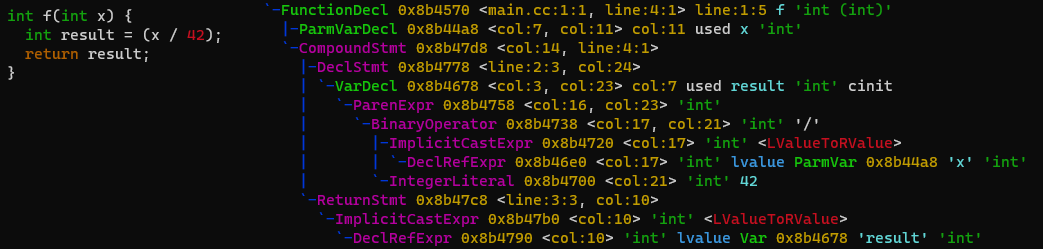
\includegraphics[width=\textwidth]{images/AST_example.png}
	\caption{Clang AST example}
	\label{fig:clang-ast}
\end{figure}


Although AST matching is clearly superior to Textual Pattern Matching, snippet \ref{src:pos34ast} demonstrates that POS34 is a control flow dependent problem that cannot be solved using this technique.
Similar arguments can be made for the other two rules. 



\lstset{caption={POS34 depends on control flow}, label=src:pos34ast}
\begin{lstlisting}[language={C++}]
void foo() {
    char *buffer = "X=Y";
    if (rand() % 2 == 0) {
        buffer = malloc(4);
        strcpy(buffer, "X=Y");
    }
    putenv(buffer); // is buffer on heap or stack?
}
void bar() {
    char *buffer = malloc(4);
    strcpy(buffer, "X=Y");
    if (rand() % 2 == 0) {
        free(buffer);
        buffer = "X=Y";
    }
    putenv(buffer); // is buffer on heap or stack?
}

\end{lstlisting}

\subsubsection{Symbolic Execution}
The Symbolic Execution technique simulates program execution, tries to enumerate every possible execution path, and assigns symbols to represent unknown values. It stores the constraints on symbols (see figure \ref{fig:state}) and eliminates unreachable paths. Such an execution comes at a high cost (exponential in the worst case), but it produces very precise results and allows for the detection of more complex bugs.


\begin{figure}[H]
	\centering
	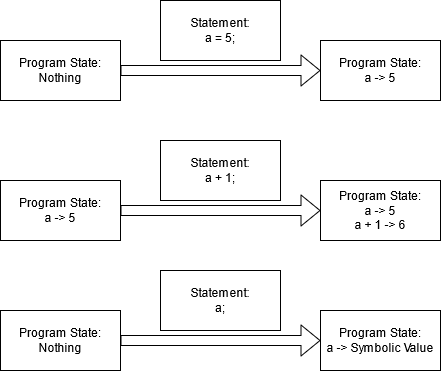
\includegraphics[width=0.6\textwidth]{images/EG.png}
	\caption{How statements affect the program state}
	\label{fig:state}
\end{figure}



\subsection{Clang Static Analyzer}
Clang Static Analyzer is a sophisticated, modern automated tool for detecting flaws in C, C++, and Objective-C codebases.
It is included in the Clang compiler and makes use of all of LLVM's algorithms and data structures. 

The tool is developed and used by technology giants like Ericsson, Apple, Google, Microsoft, Mozilla, and others together with the open-source community and academia.
Clang SA is a path-sensitive analyzer that also performs symbolic execution, has excellent memory modeling \cite{memorym}, and is context-sensitive.
All of this enables Clang Static Analyzer to detect more sophisticated problems, such as bad sequences of events in your program.

Finding the bug is only part of the analyzer's job; equally important is how the tool communicates the report to the developer, especially if it is the result of a long chain of events. 
Clang SA displays the full path, how the problem could have occurred. Figure \ref{fig:div-by-zero} shows analysis result for the Code \ref{src:simple-example}.

Furthermore, the tool is extensible by implementing new modules known as checkers \cite{llvm-dev-meeting}, allowing us to detect new types of bugs.

All of these factors combine to make Clang Static Analyzer an ideal tool for this project. 


\lstset{caption={Invalidated pointer usage.}, label=src:simple-example}
\begin{lstlisting}[language={C++}]
int foo(int x) {
    int y = x;
    if (y == 0) {
        return 1/x;
    }
    return 0;
}

\end{lstlisting}

\begin{figure}[H]
	\centering
	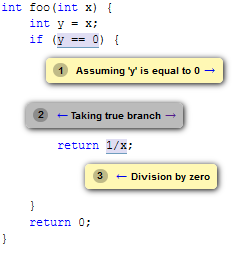
\includegraphics[width=0.6\textwidth]{images/division_by_zero_report.PNG}
	\caption{Static Analyzer warning example}
	\label{fig:div-by-zero}
\end{figure}

